%%%%%%%%%%%%%%%%%%%%%%%%%%%%%%%%%%%%%%%%%%%%%%%%%%%%%%%%%%%%%%%%%%%%
% Diskussion und Ausblick
%%%%%%%%%%%%%%%%%%%%%%%%%%%%%%%%%%%%%%%%%%%%%%%%%%%%%%%%%%%%%%%%%%%%
\onehalfspacing
\chapter{Outlook}
  \label{Outlook}

\section{Trello Alfred Extension}\index{Trello}\index{Alfred!Extension}

Alfred \index{Alfred} is a small Mac\index{Mac} application which simplifies the way one can search the web or access all sorts of applications. It simply consists of an input field which one can access with a keystroke combination. It is alike to an extended Spotlight (on Mac\index{Mac}) or Windows Search\index{Windows!Search} (on Windows). Developers can write extensions to access other web services and applications with Alfred\index{Alfred}. It even is possible to run scripts with Alfred\index{Alfred}. With that possibility given, it is perfect for accessing Trello while working in a fast and easy way. \cite{alfred}



There are three commands to add or read cards with this extension:

\begin{enumerate}
	\item \texttt{trello [board-name]} will return the card-names and statuses of this board.
	\item \texttt{trello [board-name] [list-name]} will return card-names and statuses of this list in this board.
	\item \texttt{trello [board-name] [text for a new card]} will add a new card with the specified text to the first list of this board.
	\item \texttt{trello [board-name] [list-name] [text for a new card]} will add a new card with the specified text to this list of this board.
\end{enumerate}

If you enter \texttt{trello Berlin Visit the Reichstag} in Alfred\index{Alfred}, the extension looks for a board called \emph{Berlin}. If it finds nothing, it looks for \emph{Berlin Visit} and so forth. It is therefore advisable for board names to not end on an imperative. The thought behind this operating principle is that it's very unlikely for a board name to end on an imperative and that imperatives are often used for card titles because cards are generally phrased as a command to oneself.

\begin{figure}[htb]
\centering
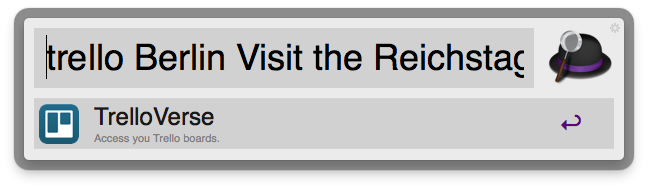
\includegraphics[width=\textwidth]{figures/trello-ext.png}
\caption{Alfred Extension\index{Alfred!Extension} for Trello\index{Trello}: This command would add a card with the name \emph{Visit the Reichstag} to the board called \emph{Berlin}.}
\label{fig:trello-ext}
\end{figure}

If you omit the text after the board name, the extension will show you all card names of this board and their statuses.

Sometimes, there are several boards with similar names. In this case, the extension will pick the \textquotedblleft last\textquotedblright match. If you have two boards called \emph{Berlin} and \emph{Berlin sightseeing}, the extension will pick \emph{Berlin sightseeing}. This approach makes sense considering that, if the extension would pick the first match -- in this case \emph{Berlin} -- it wouldn't be possible at all to access \emph{Berlin sightseeing}. When aiming to access \emph{Berlin} and add a new card beginning with \emph{sightseeing}, one has to put this board name between tick marks.

\section{Native applications}
Although Trello is an extremely good web-app, I'm convinced that a native application is always the better solution. Firstly, it is a dedicated app and therefore integrated with the operating system. Especially for todo-applications, it is favourable to be able to access the system's notification system. This way, the application can stay invisible in the background until the user actually needs to be alerted, thus granting an undisturbed working environment. There are mobile applications for iOS\index{iOS} \cite{trello:ios} and Android\index{Android} \cite{trello:android} by Trello itself, but there is no Mac\index{Mac}, Windows\index{Windows}, or Linux\index{Linux} application.

A native application would even speed up the Alfred\index{Alfred} extension because it could cache the data. This way, there wouldn't be a need for an actual HTTP request for every command by the Alfred extension. And, if a HTTP request is necessary, the user doesn't have to wait as the application will handle the command in the background.

\section{New interesting methods}
During the period of this thesis Trello introduced several new features and API calls. Some of them couldn't be considered in the thesis, for time reasons.

\subsection{Card Cover Images}
Trello introduced \emph{Card Cover Images}. \footnote{Blog post about Card Cover Images: \url{http://blog.trello.com/card-cover-images-and-drag-and-drop-attachments/}} Covers are special images, attached to a card. They are shown on the front of the card in Trello. Image attachments used as covers could have a different context than other attachments. It could be an icon to which reflects the scope of a card, for example.

\subsection{Searching}
Developers can now use the API to search\footnote{Blog post about the new Trello search: \url{https://trello.com/docs/api/search/index.html}} a Trello account. The archive can be searched, too. This function might be useful especially for desktop applications. 

\subsection{Google Drive integration}
The integration with Google Drive\footnote{Blog post about the Google Drive integration: \url{http://blog.trello.com/introducing-google-drive-integration/}} isn't an API function, yet. But if it is accessible over the API it might be an interesting feature. Desktop applications could add attachments to a Trello card and at the same time Trello uploads those attachments to Google Drive. That could be something like an automatic portfolio generator. All material for a project would be automatically saved in a directory.